% Preamble
\documentclass{article}
\usepackage[a4paper]{geometry}
\usepackage{graphicx}
\usepackage[utf8]{inputenc}
\usepackage[slovak]{babel}
\usepackage[hidelinks]{hyperref}
\usepackage{float}

\title{KONCEPTUÁLNA ANALÝZA: vizualizácia algoritmu Minimax}
\author{Stanislav Krajčovič \and Martin Maco \and Miloš Polakovič \and Vlastimil Starec}

\begin{document}
% Page title
\begin{titlepage}
	\centering
	
\includegraphics[width=20em]{images/fmfi_uk.jpg}
	\par\vspace{0.5cm}
	{\scshape\Large FAKULTA MATEMATIKY, FYZIKY A INFORMATIKY UNIVERZITA KOMENSKÉHO}
	\par\vspace{2cm}
	{\LARGE \textbf{KONCEPTUÁLNA ANALÝZA}}
	\par\vspace{0.2cm}
	{\Large vizualizácia algoritmu \textbf{Minimax}}
	\par\vfill
	Stanislav Krajčovič \quad Martin Maco \quad Miloš Polakovič \quad Vlastimil Starec
	\par\vspace{0.2cm}
	\textbf{zimný semester 2015/2016}
\end{titlepage}

% Entity relationship diagram
\begin{figure}[H]
	\centering
	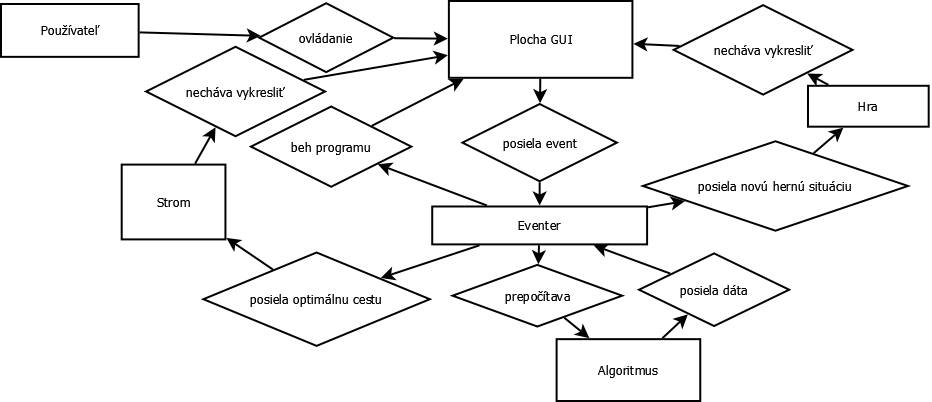
\includegraphics[width=\textwidth]{images/entity_relationship-diagram.jpg}
	\caption{Entitno-relačný diagram}
	\label{fig:entityrel}
\end{figure}
\begin{table}[H]
	\centering
	\begin{tabular}{p{8em} p{30em}}
	Používateľ (profesor, študent) &
	ovláda aplikáciu $\rightarrow$  hrá proti počítaču alebo necháva hrať počítač sám so sebou, môže si vyžiadať ďalší krok, môže pozastaviť výpočet \\ \\
	Plocha GUI &
	prijíma vstupy od používateľa a posiela ich do Eventeru, prijíma vstupy z rôznych komponentov na vykreslenie \\ \\
	Strom &
	súčasť GUI, ilustruje algoritmus ... prijíma dáta z Eventeru a necháva ich vykresliť do Plochy GUI \\ \\
	Hra &
	súčasť GUI, ilustruje aktuálny stav hry ... prijíma dáta z Eventeru a necháva ich vykresliť do Plochy GUI \\ \\
	Algoritmus &
	samotná "skrytá" časť kódu ... dostane impulz z Eventera, spracúva dáta a posiela ich späť \\ \\
	Eventer &
	najdôležitejšia skrytá komunikačná entita ... spracúva eventy do užívateľa a algoritmu, podľa nich komunikuje s algoritmom, ovládaním plochy alebo vykreslenia Hry a Stromu \\ \\
	\end{tabular}
	\caption{\nameref{fig:entityrel} - vysvetlivky}
\end{table}
\newpage

% Use case diagram
\begin{figure}[H]
	\centering
	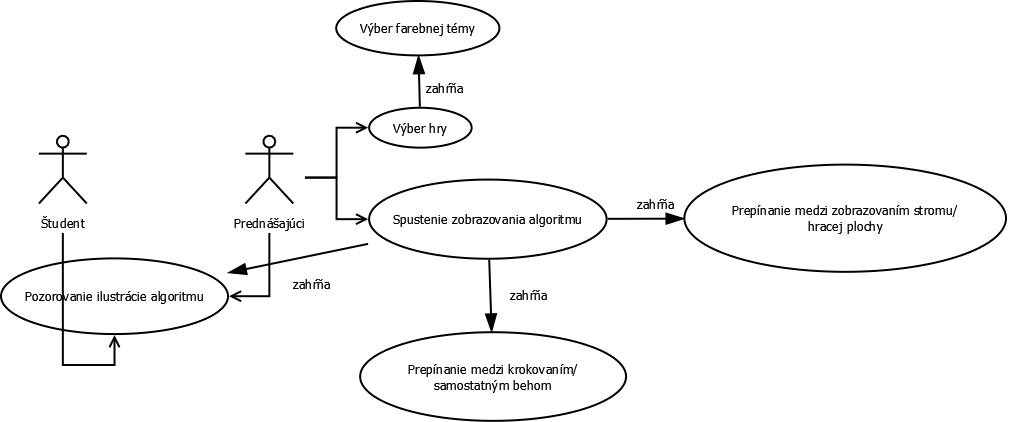
\includegraphics[width=\textwidth]{images/use_case-diagram.jpg}
	\caption{Use case diagram}
	\label{fig:usecase}
\end{figure}
\nameref{fig:usecase} ilustruje jednotlivé prípady použitia systému z pohľadu jeho používateľov. Ilustruje \emph{prednášajúceho} ako hlavného riadiaceho na aplikáciu a \emph{študenta}, ktorý je len pozorovateľ. \nameref{fig:usecase} veľmi pekne predstavuje vzťah medzi \emph{aktérmi} (\emph{študent} a \emph{prednášajúci}, v tomto prípade) a užívateľským rozhraním (Výber hry, Výber farebnej témy, ...).

% State diagram
\begin{figure}[H]
	\centering
	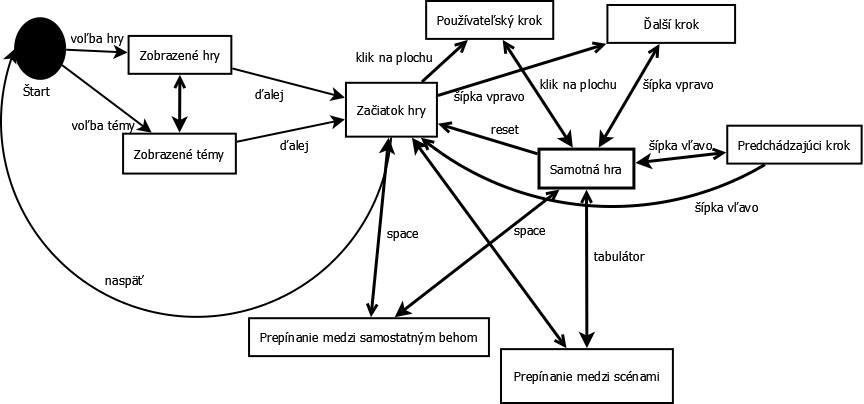
\includegraphics[width=\textwidth]{images/state-diagram.jpg}
	\caption{Stavový diagram}
	\label{fig:state}
\end{figure}
V aplikácii rozoznávame dva hlavné stavy: nastavenie hry a samotná hra.
Pri štarte aplikácie sa automaticky dostávame do nastavení hry - tam pomocou zobrazených tém a zobrazených hier vieme tlačidlom štart spustiť druhý stav, teda Hru. Z hry sa kedykoľvek môžeme vrátiť naspäť do nastavení. V hre rozoznávame ďalšie stavy. Pomocou medzerníku vieme prepínať medzi automatickým (rozumne časovaným) chodom hry. Pomocou tabulátora vieme graficky prioritizovať scénu - hra, strom, oboje. Šípkami vľavo a vpravo si vieme vynútiť predchádzajúci respektíve ďalší krok, pokiaľ nie je aplikácia automaticky časovaná. Splnením tejto podmienky vieme aj "hrať" proti počítaču kliknutím na hernú plochu. Tým si automaticky vyžiadame ďalší krok (odpoveď) počítača. Rozohranú hru vieme kedykoľvek reštartovať, teda vrátiť do pôvodného stavu.

% GUI graph
\begin{figure}[H]
		\centering
		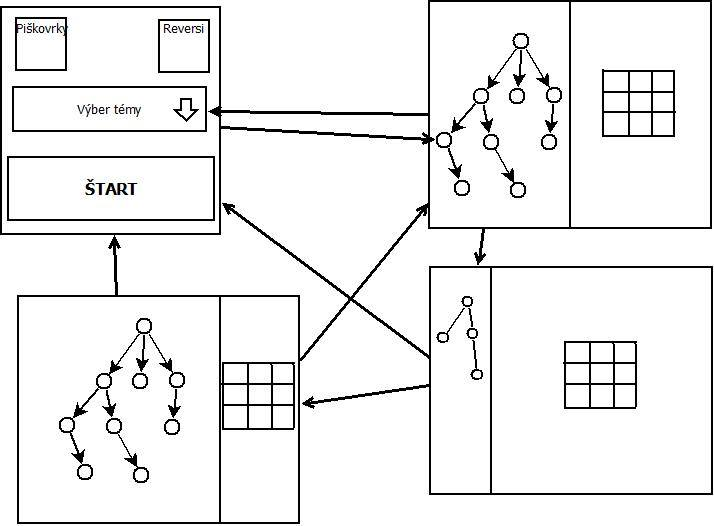
\includegraphics[width=\textwidth]{images/gui_graph-diagram.jpg}
		\caption{graf GUI}
		\label{fig:guigraph}
\end{figure}
V programe poznáme dve hlavné scény: scéna nastavení a scéna hry. Scéna nastavení vyzerá vždy rovnako. Obsahuje výber hry a vybranie grafickej témy, ktorá slúži pre adaptovanie sa publiku, teda poväčšine študentom. Z tejto scény sa pomocou tlačidla štart vieme prepnúť do druhej scény - hry. V hre poznáme tri "podscény", na ktorých je vykreslené presne to isté, avšak na každej sa kladie dôraz na niečo iné. Pri prechode z nastavení sa dostaneme na "vyrovnanú scénu". Tam nájdeme na ľavej strane strom a na pravej strane hru s ovládaním. Obe strany sú si rovné. Tabulátorom sa môžeme prepnúť do ďalšej podscény, kde raz dostaneme scénu s dôrazom na strom alebo sna hru. Z týchto podscén sa dá potom dostať späť na vyrovnanú scénu. Z hry sa kedykoľvek vieme prepnúť na scénu nastavenia.


\end{document}
